\subsection{Văn phòng số, nhiệm vụ và lịch công tác}
\label{subsec:module_ioffice}
\label{subsec:req_ioffice}
\label{subsec:req_schedule}

\subsubsection{Mục tiêu và yêu cầu chức năng}

Nhóm chức năng Văn phòng số, nhiệm vụ và lịch công tác hỗ trợ cán bộ, giảng viên tiếp cận thông tin điều hành từ hệ thống iOffice trên thiết bị di động: tra cứu văn bản đến/đi, theo dõi thông tin nhiệm vụ được giao và xem lịch làm việc tuần.

Đối với lịch công tác, MyHCMUT Mobile đóng vai trò là cổng hiển thị thống nhất (\textit{Unified Calendar}), tổng hợp các sự kiện có liên quan trực tiếp đến người dùng từ ba nguồn dữ liệu độc lập: lịch họp cơ quan từ iOffice, khoảng thời gian nghỉ phép từ HRM và các chuyến đi công tác từ HRM. Việc tổng hợp này giúp cán bộ có góc nhìn toàn diện về lịch trình cá nhân trên một giao diện duy nhất; trong đó dữ liệu nghiệp vụ gốc vẫn được quản lý và phân định thẩm quyền độc lập tại từng hệ thống nguồn.

Đối với các cuộc họp có yêu cầu điểm danh, ứng dụng hỗ trợ đại biểu ghi nhận trạng thái có mặt hoặc gửi báo vắng có lý do giải trình. Hệ thống máy chủ iOffice đóng vai trò kiểm soát độc lập các điều kiện nghiệp vụ: đại biểu phải có tên trong danh sách mời, cuộc họp đã được kích hoạt tính năng điểm danh và thời điểm thao tác phải nằm trong khung thời gian hợp lệ do ban tổ chức cấu hình.

Bảng~\ref{tab:fr_ioffice_schedule} tổng hợp các yêu cầu chức năng của nhóm nghiệp vụ này.

\begin{table}[H]
\centering
\small
\caption{Yêu cầu chức năng nhóm Văn phòng số, nhiệm vụ và lịch công tác}
\label{tab:fr_ioffice_schedule}
\begin{tabularx}{\textwidth}{|L{1.8cm}|L{3.5cm}|L{2.5cm}|Y|}
\hline
\textbf{Mã FR} & \textbf{Chức năng} & \textbf{Tác nhân} & \textbf{Mô tả và ràng buộc nghiệp vụ} \\
\hline
FR-OFF-01 & Tra cứu văn bản đến và đi & Cán bộ, Giảng viên & Xem danh sách văn bản, tìm kiếm, lọc theo mức độ khẩn và xem tài liệu số đính kèm theo quyền. \\
\hline
FR-OFF-02 & Tra cứu thông tin nhiệm vụ & Cán bộ, Lãnh đạo & Tra cứu danh sách nhiệm vụ được giao hoặc giao đi và xem thông tin được cấp quyền, như trạng thái hoặc hạn xử lý. \\
\hline
FR-SCH-01 & Điểm danh và báo vắng & Cán bộ (Đại biểu) & Ghi nhận có mặt hoặc báo vắng có lý do trong khung thời gian và điều kiện hợp lệ. \\
\hline
FR-SCH-02 & Xem lịch công tác tổng hợp & Cán bộ, Giảng viên & Hiển thị lịch tuần tổng hợp từ 3 nguồn: lịch họp iOffice, lịch phép HRM và lịch công tác HRM. \\
\hline
\end{tabularx}
\end{table}

\subsubsection{Đặc tả Use Case}

Các use case của nhóm chức năng này tập trung vào mục tiêu tra cứu văn bản, theo dõi thông tin nhiệm vụ, xem lịch công tác tổng hợp và thực hiện điểm danh cuộc họp. Hình~\ref{fig:uc_ioffice_schedule} thể hiện sơ đồ use case của nhóm này.

\begin{figure}[H]
\centering
\fbox{\parbox[c][5.5cm][c]{0.85\linewidth}{\centering \textbf{Sơ đồ Đặc tả Use case Văn phòng số, Nhiệm vụ và Lịch công tác} \newline \textit{(Gồm tác nhân Cán bộ/Giảng viên, Đại biểu cuộc họp và các use case UC-OFF-01, UC-SCH-01, UC-SCH-02)}}}
\caption{Sơ đồ Đặc tả Use case nhóm Văn phòng số, nhiệm vụ và lịch công tác}
\label{fig:uc_ioffice_schedule}
\end{figure}

Bảng~\ref{tab:mapping_uc_ioffice} tổng hợp danh mục các use case thuộc nhóm chức năng này.

\begin{table}[H]
\centering
\small
\caption{Danh mục Đặc tả Use case nhóm Văn phòng số, nhiệm vụ và lịch công tác}
\label{tab:mapping_uc_ioffice}
\vspace{0.15cm}
\begin{tabularx}{\textwidth}{|L{2.6cm}|L{4.5cm}|Y|}
\hline
\textbf{Mã Use Case} & \textbf{Tên Use Case} & \textbf{Mục tiêu Nghiệp vụ} \\
\hline
\textbf{UC-OFF-01} & Tra cứu văn bản và nhiệm vụ & Tra cứu văn bản đến/đi, xem tệp đính kèm và theo dõi thông tin các nhiệm vụ được giao trong phạm vi quyền truy cập. \\
\hline
\textbf{UC-SCH-01} & Điểm danh hoặc báo vắng cuộc họp & Ghi nhận có mặt hoặc báo vắng kèm lý do khi tham dự cuộc họp có cấu hình điểm danh. \\
\hline
\textbf{UC-SCH-02} & Xem lịch công tác tổng hợp & Xem các sự kiện từ 3 nguồn dữ liệu (lịch họp iOffice, lịch phép HRM, lịch công tác HRM). \\
\hline
\end{tabularx}
\end{table}

Đặc tả Use casecó nhiều điều kiện nghiệp vụ đáng chú ý là \textbf{UC-SCH-01} được đặc tả chi tiết tại Bảng~\ref{tab:uc_sch_01}. Các use case \textbf{UC-OFF-01} và \textbf{UC-SCH-02} được đặc tả tại Bảng~\ref{tab:uc_off_01} và Bảng~\ref{tab:uc_sch_02}.

\usecasespec{
  id={UC-OFF-01},
  name={Tra cứu văn bản và nhiệm vụ},
  shortname={Tra cứu văn bản \& nhiệm vụ},
  actor={Cán bộ / Giảng viên, Lãnh đạo Đơn vị},
  desc={Cho phép người dùng tra cứu văn bản đến/đi, xem tệp đính kèm và theo dõi thông tin các nhiệm vụ được giao trong phạm vi quyền hạn.},
  pre={Người dùng đã đăng nhập thành công vào ứng dụng MyHCMUT Mobile.},
  trigger={Người dùng chọn mục ``Văn bản'' hoặc ``Nhiệm vụ'' trên ứng dụng.},
  mainflow={
    1. Người dùng mở danh sách văn bản (hoặc nhiệm vụ) trên ứng dụng. \newline
    2. Hệ thống hiển thị danh sách các mục theo quyền truy cập của tài khoản. \newline
    3. Người dùng lọc theo phân loại, trạng thái hoặc tìm kiếm theo từ khóa tiêu đề. \newline
    4. Chọn xem chi tiết một văn bản (hoặc nhiệm vụ) cụ thể để kiểm tra thông tin được cấp quyền.
  },
  altflow={
    - \textit{Luồng 4a (Xem tệp tài liệu số):} Người dùng chọn mở tệp PDF đính kèm để đọc trực tiếp trên ứng dụng.
  },
  exflow={
    - \textit{Ngoại lệ 4a (Không có quyền xem tệp đính kèm):} Hệ thống thông báo văn bản bảo mật và giới hạn quyền truy cập tệp.
  },
  post={Người dùng nắm bắt được thông tin văn bản và nhiệm vụ được cấp quyền truy cập.},
  label={tab:uc_off_01}
}

\usecasespec{
  id={UC-SCH-01},
  name={Điểm danh hoặc báo vắng cuộc họp},
  shortname={Điểm danh cuộc họp},
  actor={Cán bộ / Giảng viên có tên trong danh sách mời},
  desc={Cho phép đại biểu ghi nhận có mặt hoặc báo vắng kèm lý do giải trình đối với cuộc họp có cấu hình điểm danh.},
  pre={Người dùng đã đăng nhập, có tên trong danh sách mời và cuộc họp được cấu hình tính năng điểm danh.},
  trigger={Người dùng mở màn hình chi tiết cuộc họp trên ứng dụng di động.},
  mainflow={
    1. Người dùng mở xem chi tiết cuộc họp trên giao diện Lịch hoặc từ thông báo nhắc việc. \newline
    2. Ứng dụng hiển thị các thao tác điểm danh phù hợp với trạng thái cuộc họp. \newline
    3. Người dùng chọn điểm danh có mặt hoặc báo vắng và nhập lý do khi cần. \newline
    4. Ứng dụng gửi yêu cầu đến iOffice; iOffice kiểm tra tính hợp lệ của đại biểu, cuộc họp và khung thời gian cho phép. \newline
    5. iOffice ghi nhận kết quả và phản hồi trạng thái tham dự mới để ứng dụng cập nhật thông tin hiển thị.
  },
  altflow={
    - \textit{Luồng 3a (Chuyển đổi trạng thái):} Trong khung giờ hợp lệ, người dùng có thể cập nhật lại giữa trạng thái có mặt và báo vắng.
  },
  exflow={
    - \textit{Ngoại lệ 4a (Ngoài khung thời gian):} Thao tác thực hiện ngoài khung giờ quy định $\rightarrow$ hệ thống từ chối và thông báo lý do. \newline
    - \textit{Ngoại lệ 4b (Không thuộc danh sách mời):} Người dùng không có tên trong danh sách đại biểu $\rightarrow$ hệ thống từ chối thao tác.
  },
  post={Trạng thái tham dự được ghi nhận và kết quả mới được phản hồi trên ứng dụng.},
  label={tab:uc_sch_01}
}

\usecasespec{
  id={UC-SCH-02},
  name={Xem lịch công tác tổng hợp},
  shortname={Xem lịch tổng hợp},
  actor={Cán bộ / Giảng viên},
  desc={Cho phép người dùng theo dõi lịch họp iOffice, lịch nghỉ phép HRM và lịch công tác HRM trên một giao diện tuần duy nhất.},
  pre={Người dùng đã đăng nhập và có quyền truy cập dữ liệu nguồn tương ứng.},
  trigger={Người dùng mở màn hình Lịch công tác trên ứng dụng di động.},
  mainflow={
    1. Người dùng mở mục ``Lịch công tác'' trên ứng dụng. \newline
    2. Ứng dụng đồng thời tải các sự kiện lịch mà người dùng được phép xem từ hệ thống iOffice và HRM. \newline
    3. Ứng dụng hiển thị các sự kiện trên giao diện lịch tuần thống nhất, phân biệt rõ nguồn dữ liệu qua màu sắc và nhãn phân loại. \newline
    4. Người dùng chọn một sự kiện cụ thể để xem chi tiết hoặc chuyển đến màn hình nghiệp vụ liên quan.
  },
  altflow={
    - \textit{Luồng 3a (Lọc theo nguồn dữ liệu):} Người dùng có thể bật/tắt hiển thị từng nguồn lịch (chỉ xem lịch họp hoặc chỉ xem lịch phép/công tác).
  },
  exflow={
    - \textit{Ngoại lệ 2a (Không tải được đầy đủ dữ liệu lịch):} Ứng dụng thông báo trạng thái lỗi và cho phép người dùng thực hiện lại thao tác.
  },
  post={Người dùng có góc nhìn lịch trình toàn diện mà không làm thay đổi hay sai lệch dữ liệu nghiệp vụ gốc.},
  label={tab:uc_sch_02}
}

\subsubsection{Biểu đồ hoạt động}

Quy trình điểm danh và báo vắng cuộc họp có nhiều điều kiện nghiệp vụ liên quan đến người tham dự, trạng thái cuộc họp và thời gian thực hiện, do đó được lựa chọn để mô tả bằng biểu đồ hoạt động.

Hình~\ref{fig:act_attendance} mô tả quy trình điểm danh và báo vắng cuộc họp của UC-SCH-01. Quy trình bắt đầu khi người dùng truy cập một cuộc họp có hỗ trợ điểm danh. Hệ thống kiểm tra các điều kiện thực hiện trước khi cho phép người dùng ghi nhận có mặt hoặc báo vắng kèm lý do. Khi thao tác hợp lệ, trạng thái tham dự được ghi nhận và kết quả được phản hồi trên ứng dụng; trường hợp không đáp ứng điều kiện, hệ thống từ chối thao tác và thông báo nguyên nhân cho người dùng.

\begin{figure}[H]
\centering
\fbox{\parbox[c][7cm][c]{0.85\linewidth}{\centering \textbf{Vị trí biểu đồ hoạt động} \\ \textit{Điểm danh và báo vắng cuộc họp}}}
\caption{Biểu đồ hoạt động Điểm danh và báo vắng cuộc họp}
\label{fig:act_attendance}
\end{figure}

\subsubsection{Biểu đồ tuần tự}

Biểu đồ tuần tự mô tả sự tương tác ở mức logic giữa người dùng, MyHCMUT Mobile và hệ thống iOffice trong quá trình điểm danh hoặc báo vắng cuộc họp. Khi người dùng thực hiện thao tác trên ứng dụng, yêu cầu được chuyển đến hệ thống iOffice để kiểm tra các điều kiện nghiệp vụ và ghi nhận kết quả. Trạng thái tham dự sau xử lý được trả về MyHCMUT Mobile để cập nhật thông tin hiển thị cho người dùng.

Hình~\ref{fig:seq_attendance} thể hiện trình tự tương tác của use case UC-SCH-01. Biểu đồ chỉ tập trung vào sự phối hợp giữa các thành phần ở mức hệ thống; các thành phần hiện thực và cơ chế giao tiếp chi tiết được trình bày tại Chương~5.

\begin{figure}[H]
\centering
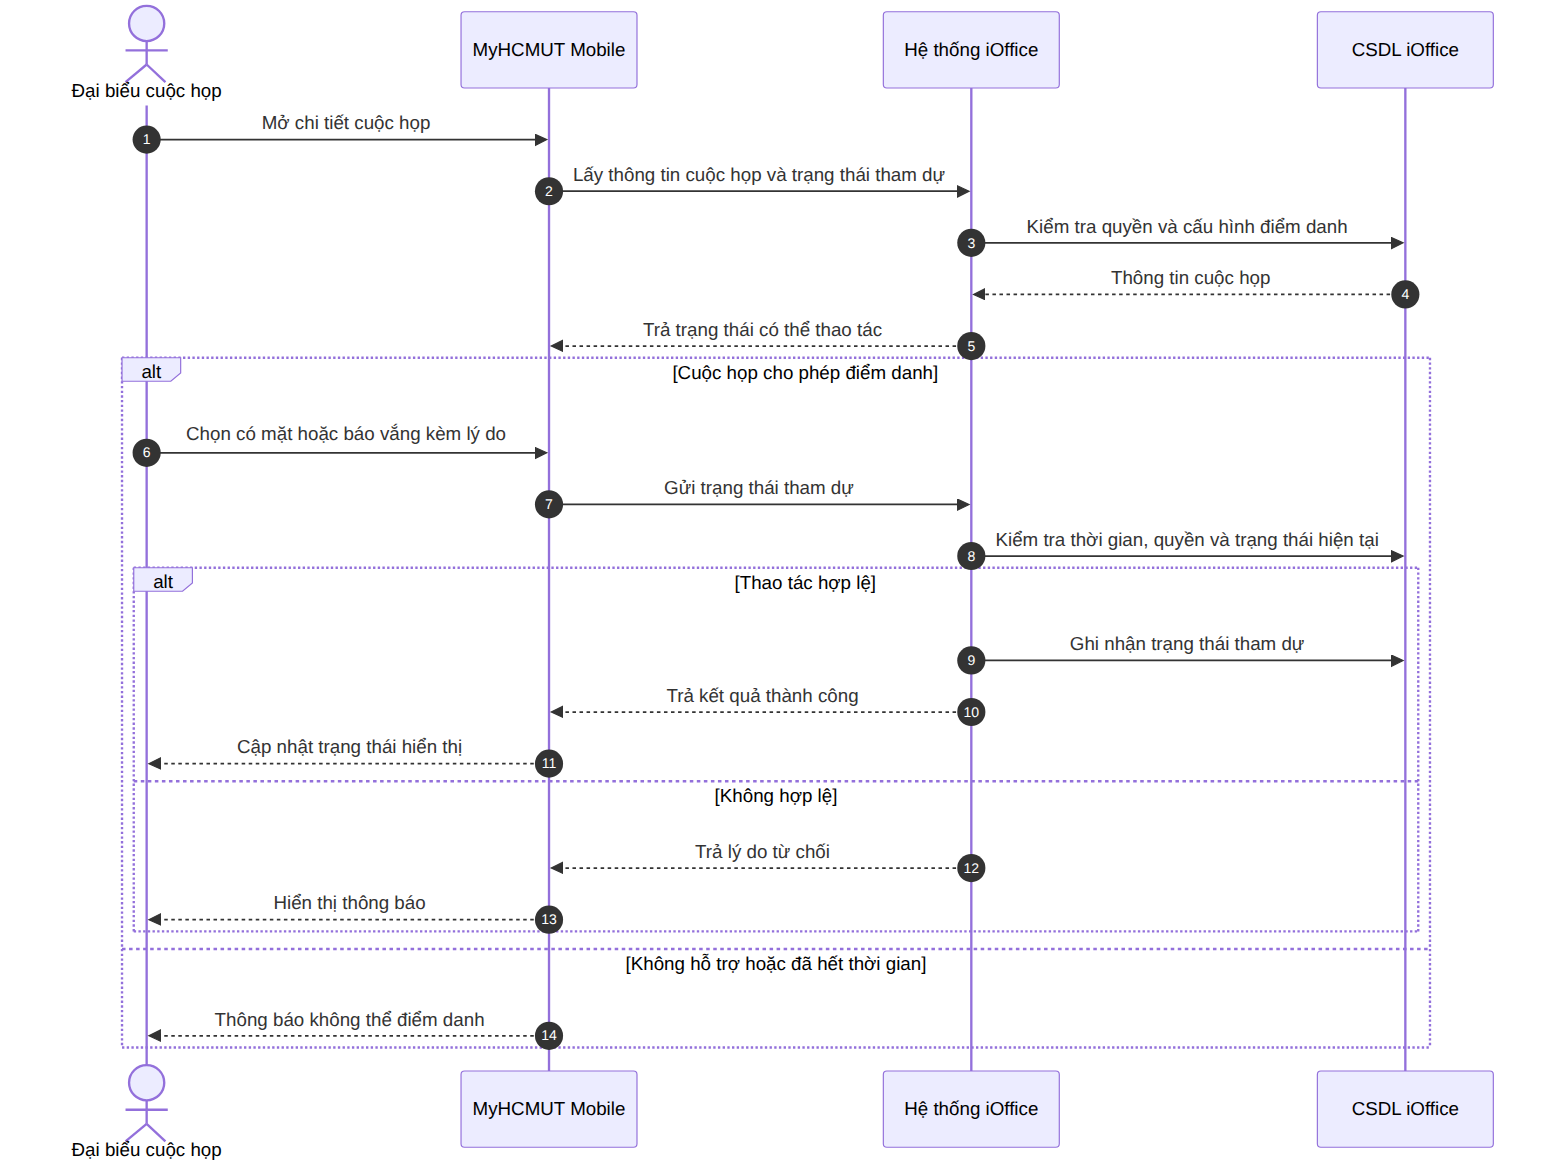
\includegraphics[width=\linewidth]{image/uml/seq_attendance.png}
\caption{Biểu đồ tuần tự Điểm danh và báo vắng cuộc họp}
\label{fig:seq_attendance}
\end{figure}
